\section{Pretty Crazy Awesome PCA \hpoints{28}}

\subsection{Classy Axes}

\begin{figure}[h!]
 \centering
 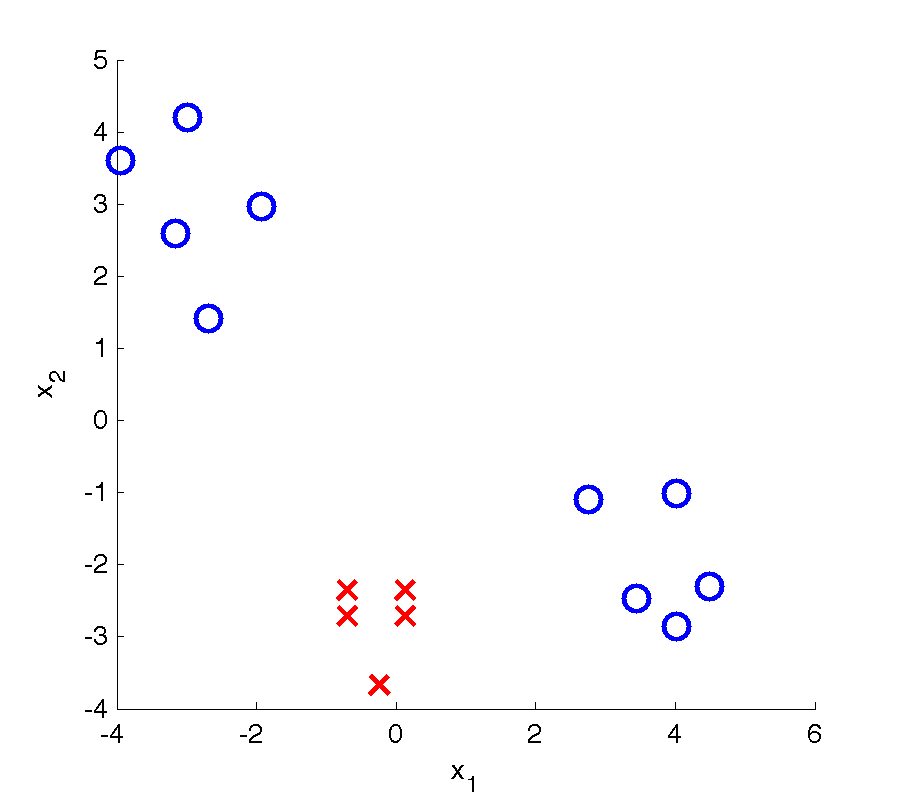
\includegraphics[width=0.43\textwidth]{images/pca_group1.png}
 \caption{Graph of Mystery.}
 \label{fig:pca1}
\end{figure}

\begin{enumerate}
\item \points{5} For the graph in Figure \ref{fig:pca1}, sketch the 2
  principal components that would be found by PCA. Label them as ``1''
  and ``2'' to indicate which is the first, and which is the second
  axis.  You don't have to precisely calculate the equations for these
  axes; you should be able to figure out which directions are the
  principal components without needing complicated formulas and draw
  lines in approximately those directions.  Remember that PCA ignores
  class labels.

\begin{figure}[h!]
 \centering
 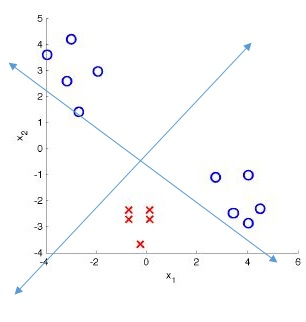
\includegraphics[width=0.43\textwidth]{images/2_1}
 \caption{Principal Components}
 \label{fig:pca3}
\end{figure}


\item \points{2} If we project the data onto a single principal
  component, which component will allow a decision stump to perfectly
  separate the data: the first, the second, or both? \\

Both \\


\item \points{2} Suppose instead we transform the data using a
  non-linear function of only one of the original axes: either
  $\phi(\bx) = x_1^2$ or $\phi(\bx) = x_2^2$. Which will allow a
  decision stump to perfectly separate the data?

 $\phi(\bx) = x_1^2$ perfectly separates the data \\

\end{enumerate}

\subsection{Like a good neighbor, PCA is there}

You showed in your first homework that nearest-neighbor classification
can suffer when many irrelevant features are present.  Here you will
show that PCA can solve this problem by analyzing the covariance
matrix of the features.  Suppose we have two classes, $y = 1, 2$, and
$P(\bx \mid y)$ is Gaussian.  For simplicity assume for all Gaussians
below that the variance $\sigma^2$ is the same.  Reminder: If $X \sim
N(\mu,\sigma^2)$, then $\E[X] = \mu$, $Var[X] = \sigma^2$, and
$\E[X^2] = \mu^2 + \sigma^2$.  Also, recall that expectation is linear
and it obeys the following four properties:
\begin{align*}
\E[X + c] =&\; \E[X] + c\;\;\; \textrm{for any constant}\; c \\
\E[X + Y] =&\; \E[X] + \E[Y] \\
\E[aX] =&\; a\E[X]\;\;\; \textrm{for any constant}\; a \\
\E[X] =&\; \E_Y [ \E_X [X \mid Y] ] \;\;\; \textrm{(iterated expectation)}
\end{align*}

\begin{align*}
& \; \text{We know that }\\
P(X) &\; = \sum\limits_k P(X,Y=k) \\
 =&\; \sum \limits_k P(X | Y=k) P(Y=k)   (Using conditional probability)\\   
=&\; \frac{1}{2} \sum \limits_k P(X | Y=k) \\
=& \; \frac{1}{2} \left( N(1 , \sigma^2) + N (-1 , \sigma^2) \right) \\
&\; Using \; X = N (\mu_1 , \sigma_1) \; and \; Y =  N (\mu_2 , \sigma_2) \\
&\; if \; Z = X + Y = N (\mu_1 +\mu_2 , \sigma_1^2 + \sigma_2^2) \\
=&\; \frac{1}{2} N (0 , 2 \sigma_2) \\
&\; \text{We know that } Var[X] = \sigma^2 \\
Var[c.X] = c^2 Var[X] \\
&\; So \; Variance= \; \frac{1}{4} Var [X]\\
=&\; \frac{\sigma^2}{2} \\
\end{align*}


\begin{enumerate}
\item \points{4} Suppose our data is generated according to a Gaussian
  mixture: first $Y$ is sampled from the set of classes $\{1, 2\}$
  with equal probability ($\frac{1}{2}$) of each class being selected,
  and then a {\em scalar} $X$ is sampled according to the Gaussian
  $P(X \mid Y)$. Let $1$ be the mean of class 1 and $-1$ be the mean
  of class 2.  What is the variance of $X$? Your answer should be in
  terms of $\sigma^2$.

The variance will remain the same since the feature is uninformative, it will have no impact on the variance \\
$Var = \frac{\sigma^2}{2}$ \\

\item \points{3} Now suppose a data point $X'$ is generated according
  to same process as above, but the feature is uninformative, so the
  mean of class 1 and 2 are both zero.  What is the variance of $X'$?
  Your answer should be in terms of $\sigma^2$.

As we saw in part 1, for uninformative feature, since the mean is 0, the variance will be $\frac{\sigma^2}{2}$ \\

\item \points{3} Suppose now we generate $X$ as in part 1 and $X'$ as
  in part 2 from a single $Y$. What is the {\em covariance} between
  $X$ and $X'?$ Recall that covariance is defined as $\E[
    (X-\E_X[X])(X'-\E_{X'}[X']) ]$.

\begin{align*}
	\E[(X-\E_X[X])(X'-\E_{X'}[X']) ] \\
	=&\;  \E \left[ X X' - \E_X [X] X' - X \E_{X'} + \E_X[X'] \E_{X'}[X'] \right] \\
	&\; We \; have \; \E[X] = \mu_1 = 0 \\
	&\; E[X'] = \mu_2 = 0 \\
	=&\; \E [X X'] \\
	=&\; \E [X] \E[X'] \\
	= 0 \\
\end{align*}

\item \points{4} Suppose we generate a dataset $(\bx_1,y_1) \dots,
  (\bx_n,y_n)$ by generating one informative feature $X_1$ as in part
  1 and $m$ non-informative features $X_2, \dots, X_{m+1}$ as in part
  2 for each example. (An example 2D dataset is shown in Figure
  \ref{fig:pca-example}.) What are the eigenvalues of the covariance
  matrix of the data? Assume that $n \rightarrow \infty$, so that the
  covariances are exactly the true covariances that you computed in
  the previous questions.  {\em Hint: The eigenvalues of a diagonal
    matrix are the diagonal entries of the matrix, and the
    eigenvectors are the standard bases $e_1 = [1 \;\; 0 \;\; 0 \;\;
      \dots \;\; 0]^\top$, etc.}

  \begin{figure}[h!]
    \centering
    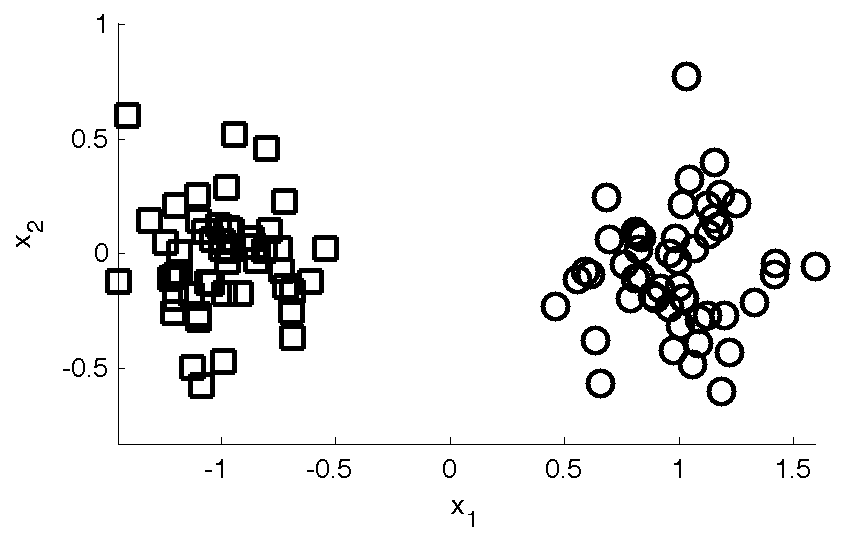
\includegraphics[width=0.6\textwidth]{images/pca_example.png}
    \caption{Sample dataset with only one informative dimension: $x_1$.}
    \label{fig:pca-example}
  \end{figure}

Since only the first feature is informative the covariance of the first feature matters\\

\item \points{3} Suppose we use a nearest-neighbor classifier on our
  data using the {\em first} principal component only.  Briefly
  explain (2-3 sentences) why the ratio of intra-class to inter-class
  distances in the space defined by the first principal component will
  increase, decrease, or not change as $m$ increases (as more
  uninformative features are added to the data). \\

No change

\item \points{2} Based on your previous answer, how will running PCA
  (and keeping only 1 component) before using K-NN affect the
  performance of K-NN as $m$ increases?  That is, will it increase,
  decrease, or have no effect on the accuracy of K-NN? \\

Increases the accuracy \\

\end{enumerate}
